\chapter{Results}\label{chap:res}

\section{Contiguous fill method results}

The following results were generated by using \verb+entropy_cont_fill+\footnote{section \ref{sec:ent_imp}} method.

\subsection{Writes: Bandwidth v/s Entropy}
\begin{figure}[H]
\begin{center}
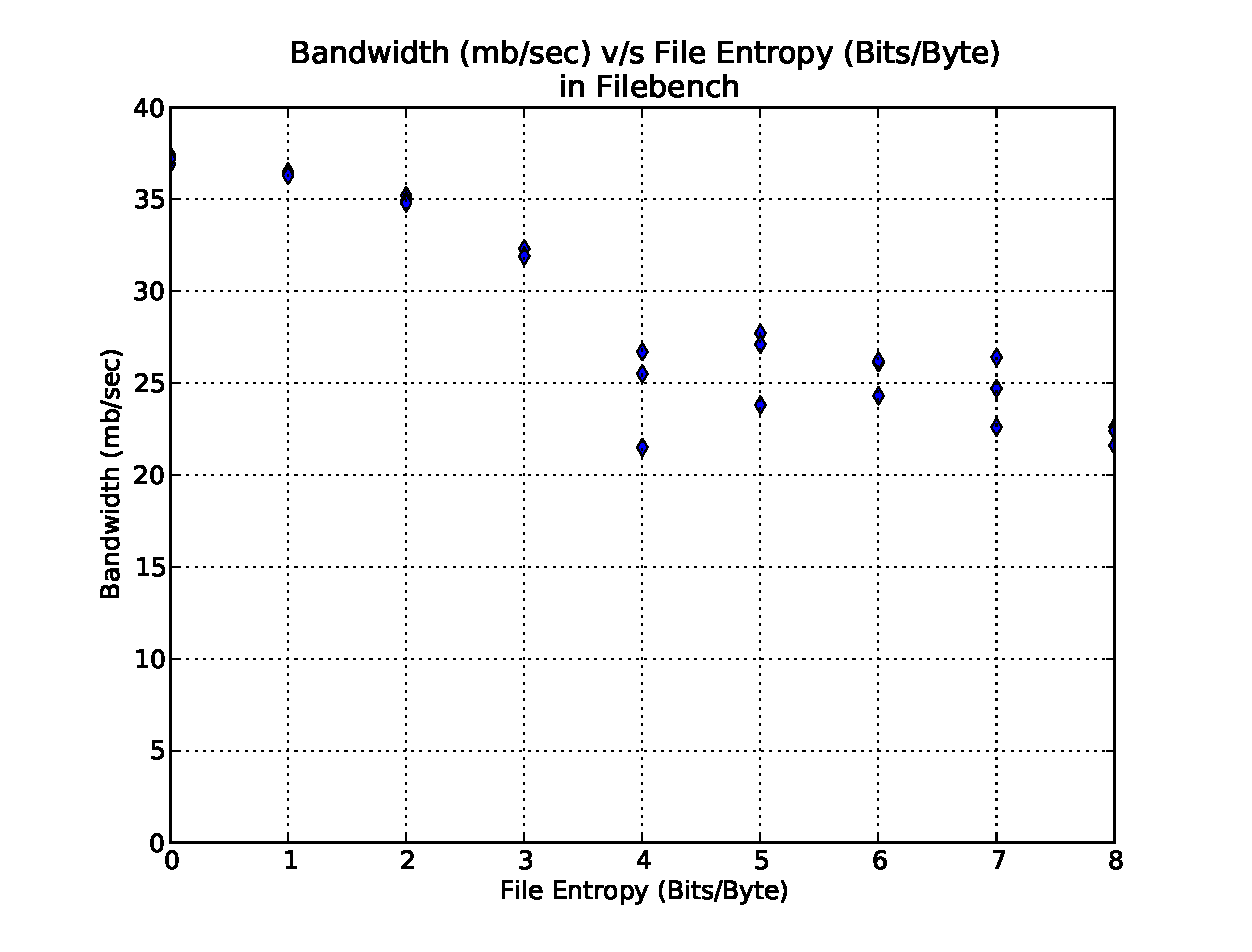
\includegraphics[scale=.55]{../results/set1/write_bw_all.eps}
\caption{The bandwidth of all the write runs}
\label{fig:wb}
\end{center}
\end{figure}

\begin{figure}[H]
\begin{center}
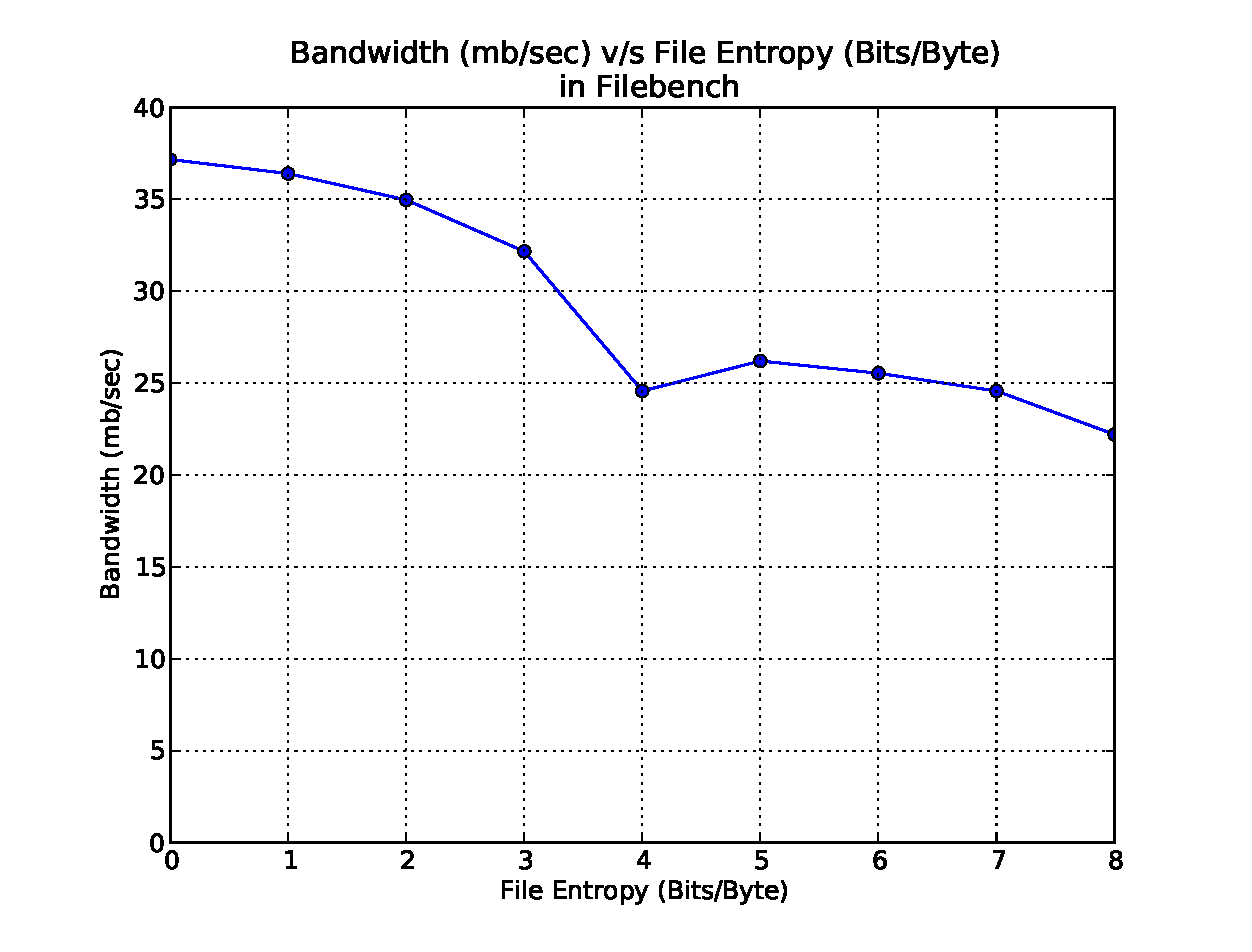
\includegraphics[scale=.55]{../results/set1/write_bw_avg.eps}
\caption{The average bandwidth over all the different write runs}
\label{fig:wbavg}
\end{center}
\end{figure}
\noindent Figures \ref{fig:wb} and \ref{fig:wbavg} show that bandwidth of the write operation is decreasing as the entropy is increased. This can be explained by the idea that the larger the entropy, the more is the "randomness" and hence, the more is the effort SDFS spends to deduplicate the files. Figure \ref{fig:wb} shows all values of bandwidth collected from 27 runs with small deviations. The average of all these runs for each entropy is calculated and presented in figure \ref{fig:wbavg}.

\subsection{Writes: Latency v/s Entropy}
\begin{figure}[H]
\begin{center}
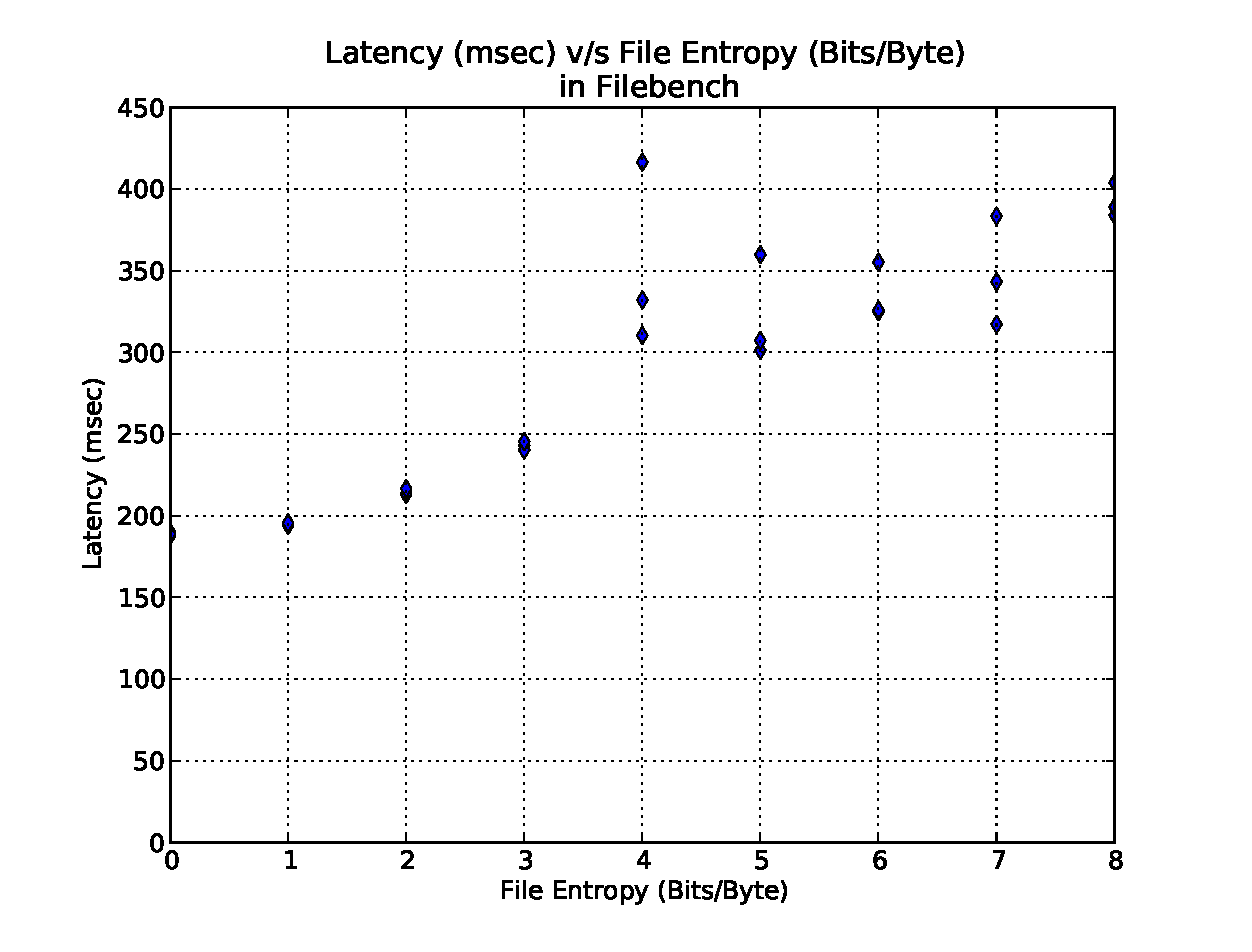
\includegraphics[scale=.55]{../results/set1/write_latency_all.eps}
\caption{The latency of all the different write runs}
\label{fig:wl}
\end{center}
\end{figure}


\begin{figure}[H]
\begin{center}
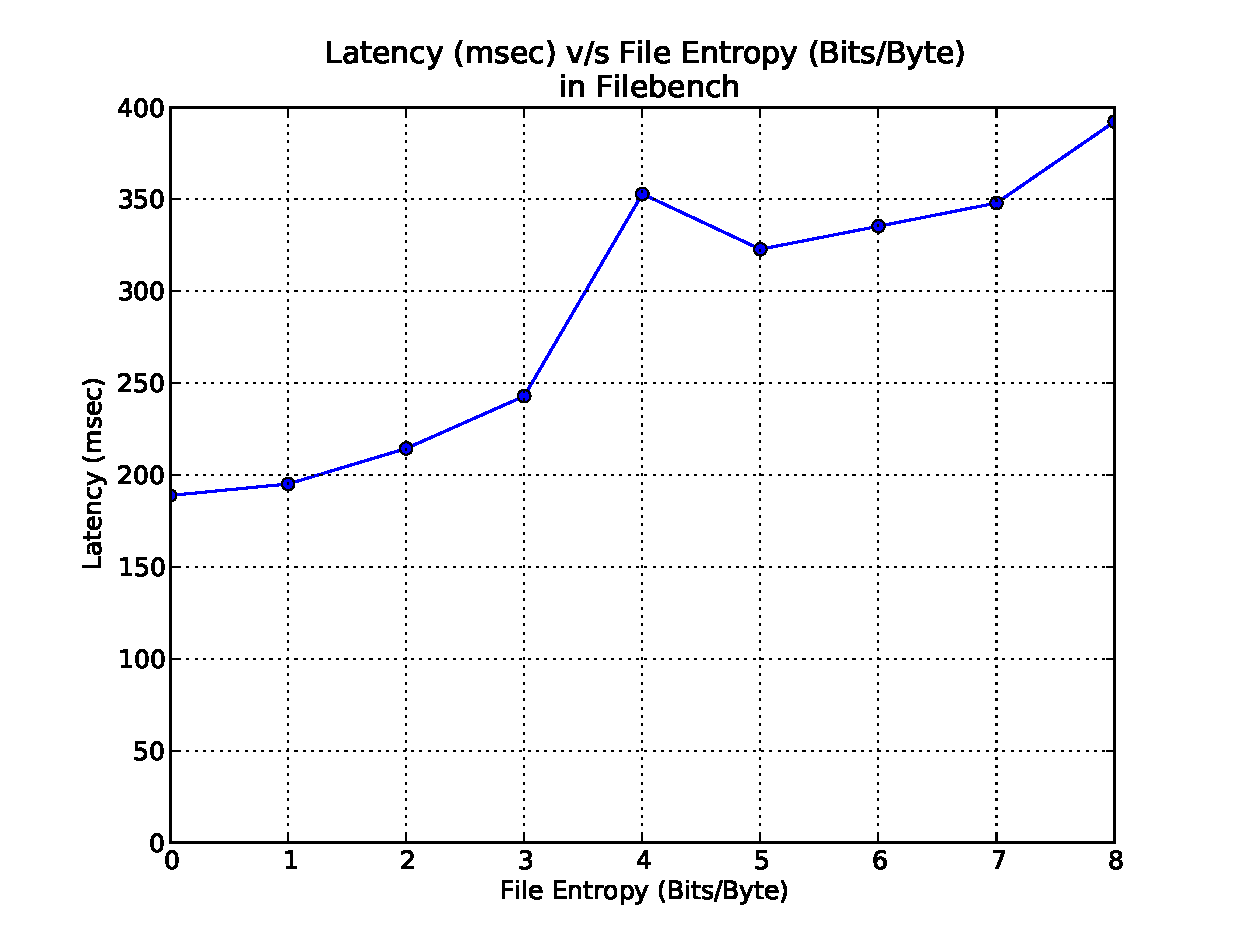
\includegraphics[scale=.55]{../results/set1/write_latency_avg.eps}
\caption{The average latency over all the write runs}
\label{fig:wlavg}
\end{center}
\end{figure}
\noindent Figures \ref{fig:wl} and \ref{fig:wlavg} show that latency of the write operation is increasing as the entropy increased. The larger the entropy the more effort that SDFS spend to deduplicate the files and the larger the latency will be for each write operation. Figure \ref{fig:wl} shows all values of latency collected from 27 runs with small deviations. The average of all these runs for each entropy is calculated and presented in figure \ref{fig:wlavg}.

\subsection{Writes: Operations/sec v/s Entropy}
\begin{figure}[H]
\begin{center}
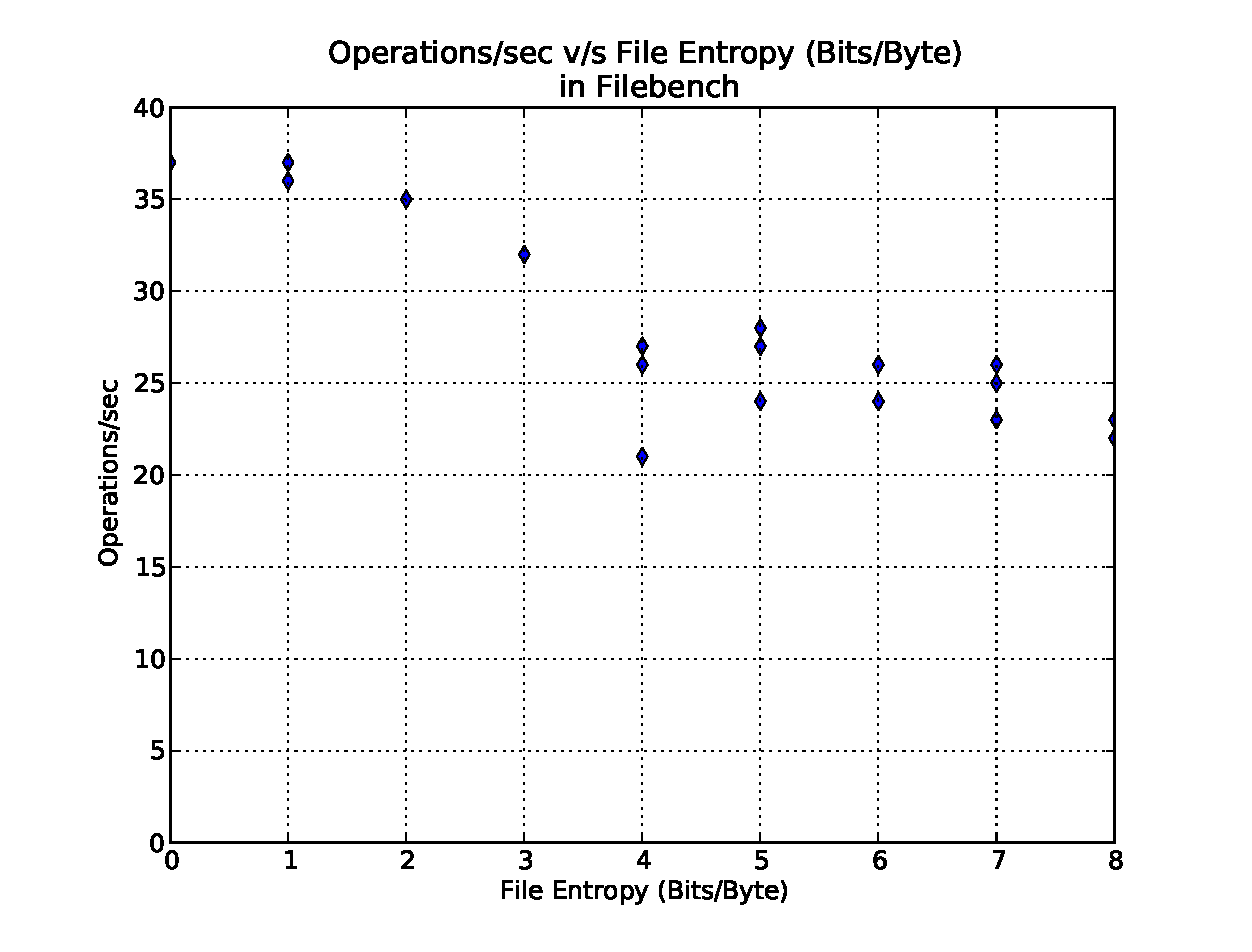
\includegraphics[scale=.55]{../results/set1/write_ops_all.eps}
\caption{The operations execution-speed of all the write runs}
\label{fig:wops}
\end{center}
\end{figure}

\begin{figure}[H]
\begin{center}
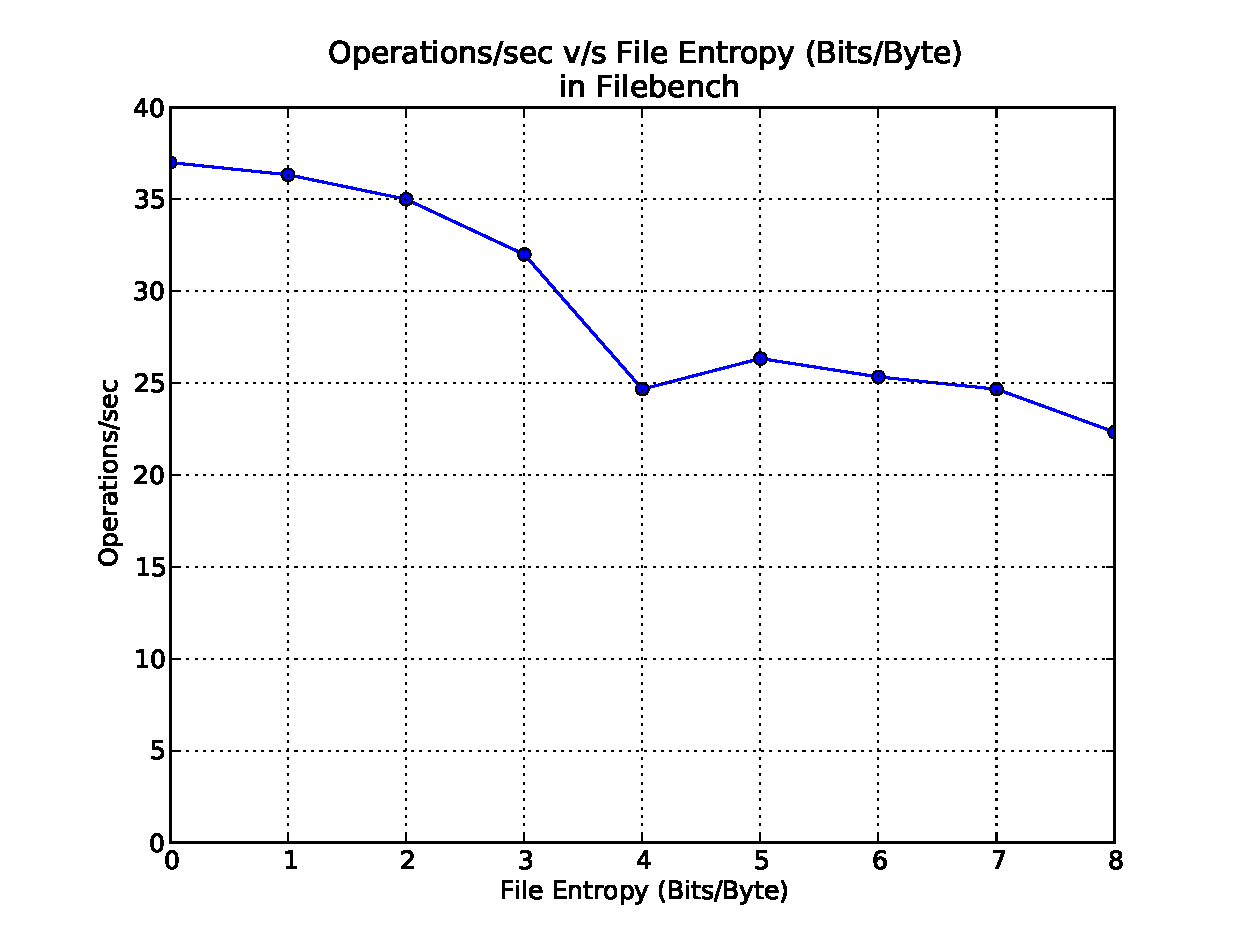
\includegraphics[scale=.55]{../results/set1/write_ops_avg.eps}
\caption{The average operations execution-speed over all the write runs}
\label{fig:wopsavg}
\end{center}
\end{figure}

\noindent The results depicted by figure \ref{fig:wops} show that the rate of operations goes down as entropy is increased. They also indicate the effect of ops/sec on bandwidth and latency. The less operations we can execute per second the less the size of data we can write which decrease the bandwidth. In the same manner if we want more time to execute a specific amount of operations, this means that the latency of the write operations is increased. Hence, these results are as expected. Figure \ref{fig:wopsavg} shows the average of the three readings obtained for each entropy value.

\subsection{Reads: Bandwidth v/s Entropy and Latency v/s Entropy}
\begin{figure}[H]
\begin{center}
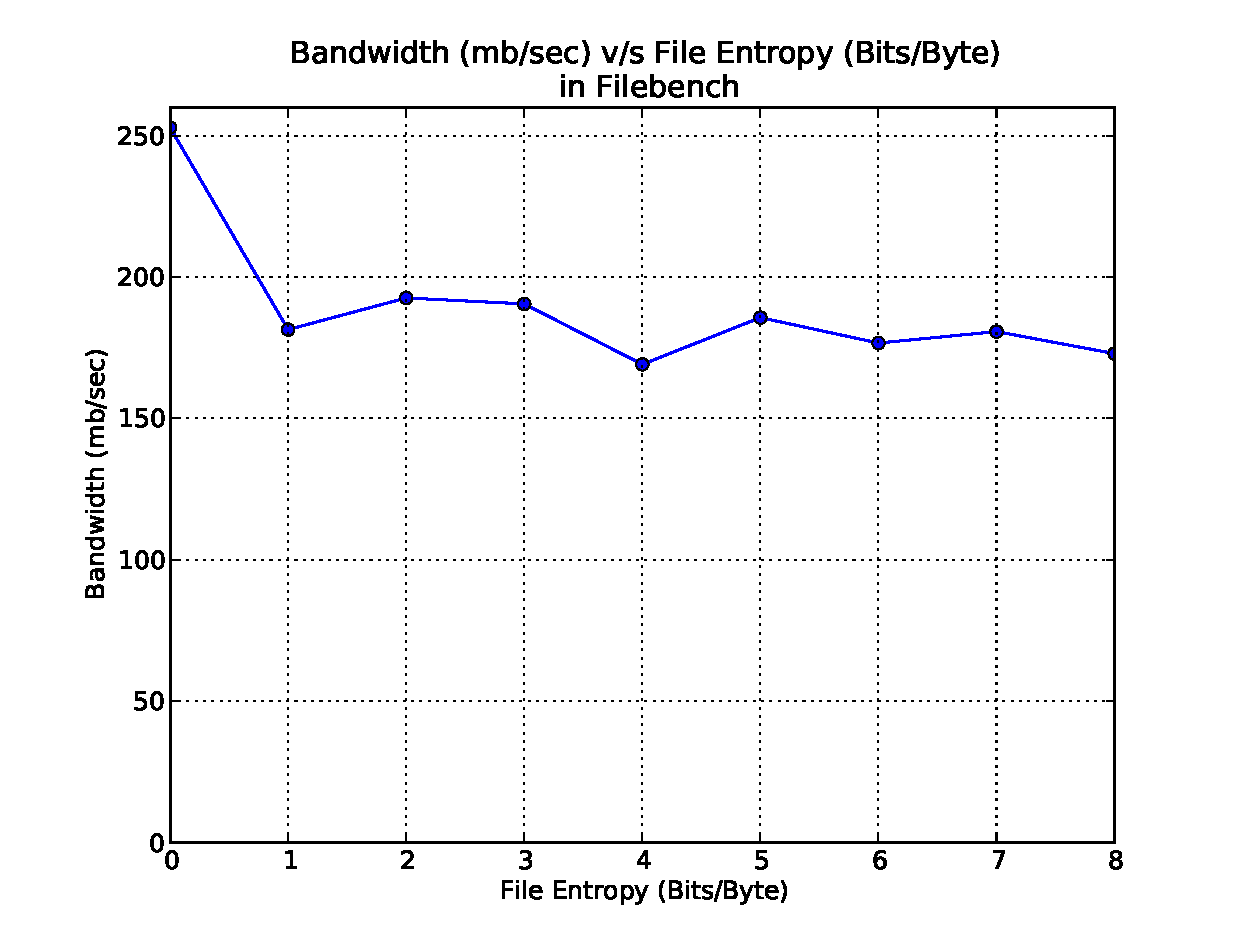
\includegraphics[scale=0.55]{../results/set1/read_bw.eps}
\caption{The bandwidth of all the read runs }
\label{fig:rb}
\end{center}
\end{figure}

\begin{figure}[H]
\begin{center}
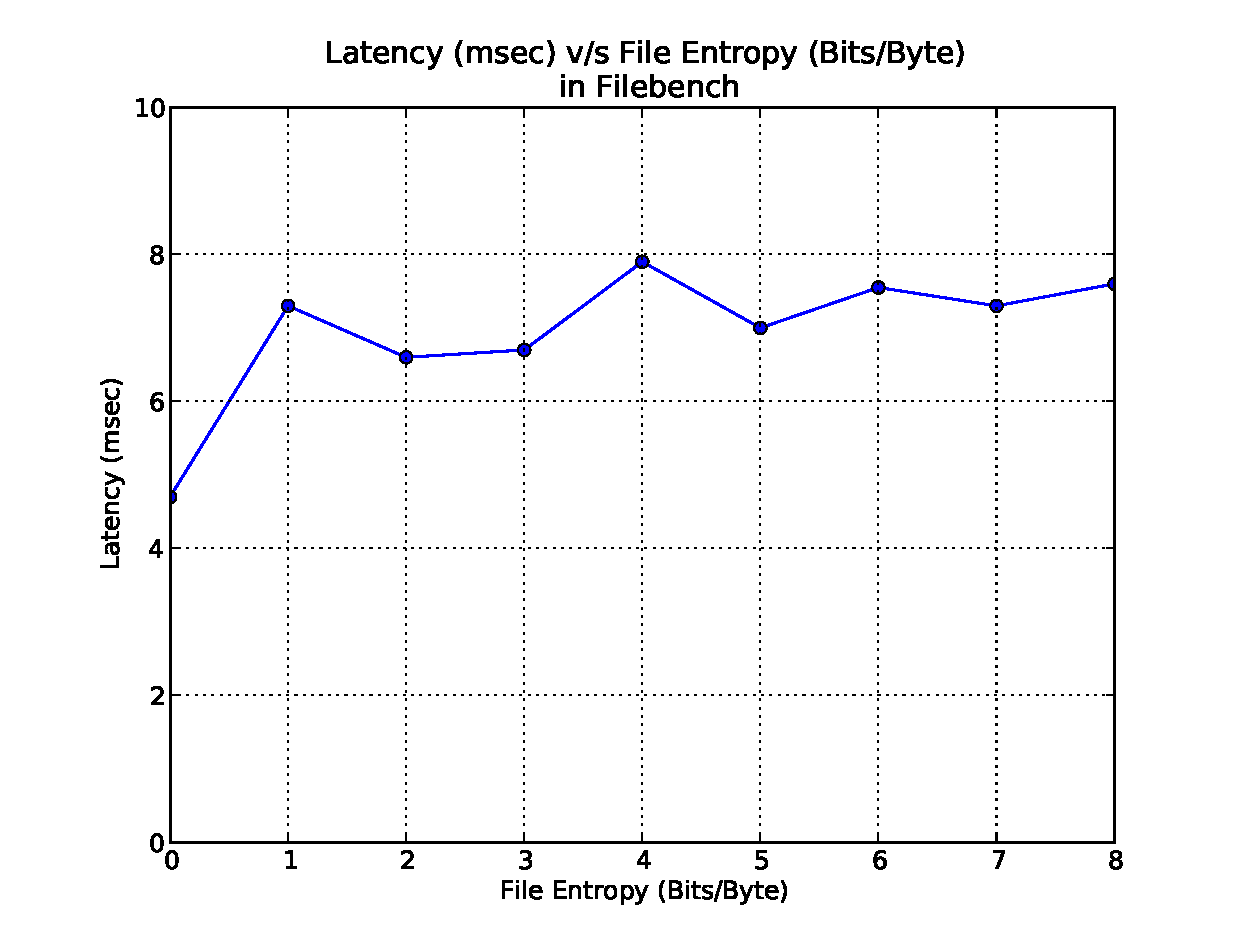
\includegraphics[scale=.55]{../results/set1/read_latency.eps}
\caption{The latency over all the read runs}
\label{fig:rl}
\end{center}
\end{figure}

\noindent The read workload preallocates around 50 GiB for each run and this takes a considerable amount of time. For this reason we could not manage to run multiple rounds of operations and then compute the average readings. We managed to run a sequence of reads with entropies 0 through 8 once, and once again from 5 through 7. Figures \ref{fig:rb} and \ref{fig:rl} show that the trends in the read workload closely follow the those of the write workload as the entropy increases.

\section{Lookup fill method results}
The following results were generated by using \verb+entropy_lookup_fill+\footnote{section \ref{sec:ent_imp}} method.

\subsection{Writes: Bandwidth v/s Entropy}
\begin{figure}[H]
\begin{center}
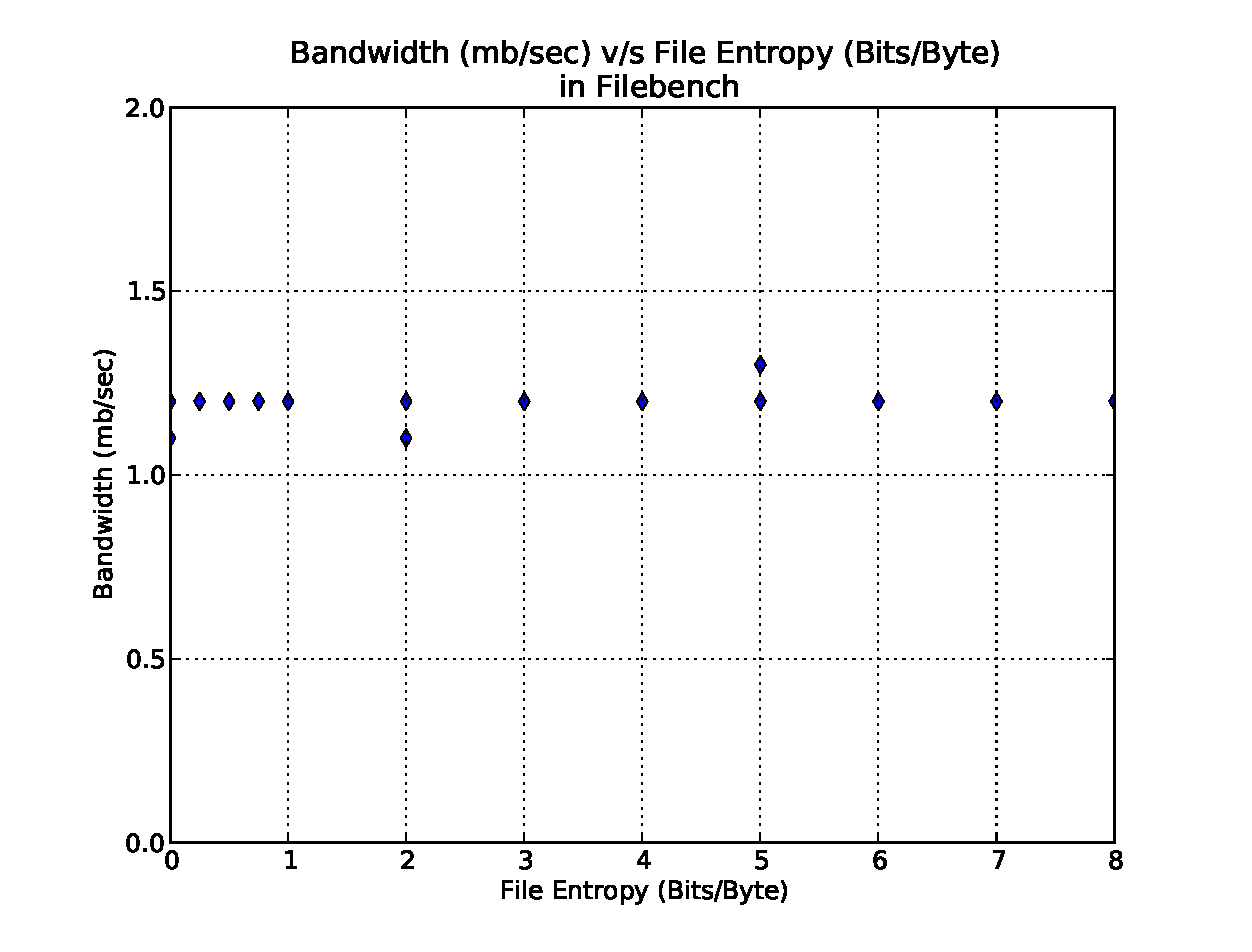
\includegraphics[scale=.55]{../results/set2/write_bw_2.eps}
\caption{The bandwidth of all the write runs}
\label{fig:wb2}
\end{center}
\end{figure}

\begin{figure}[H]
\begin{center}
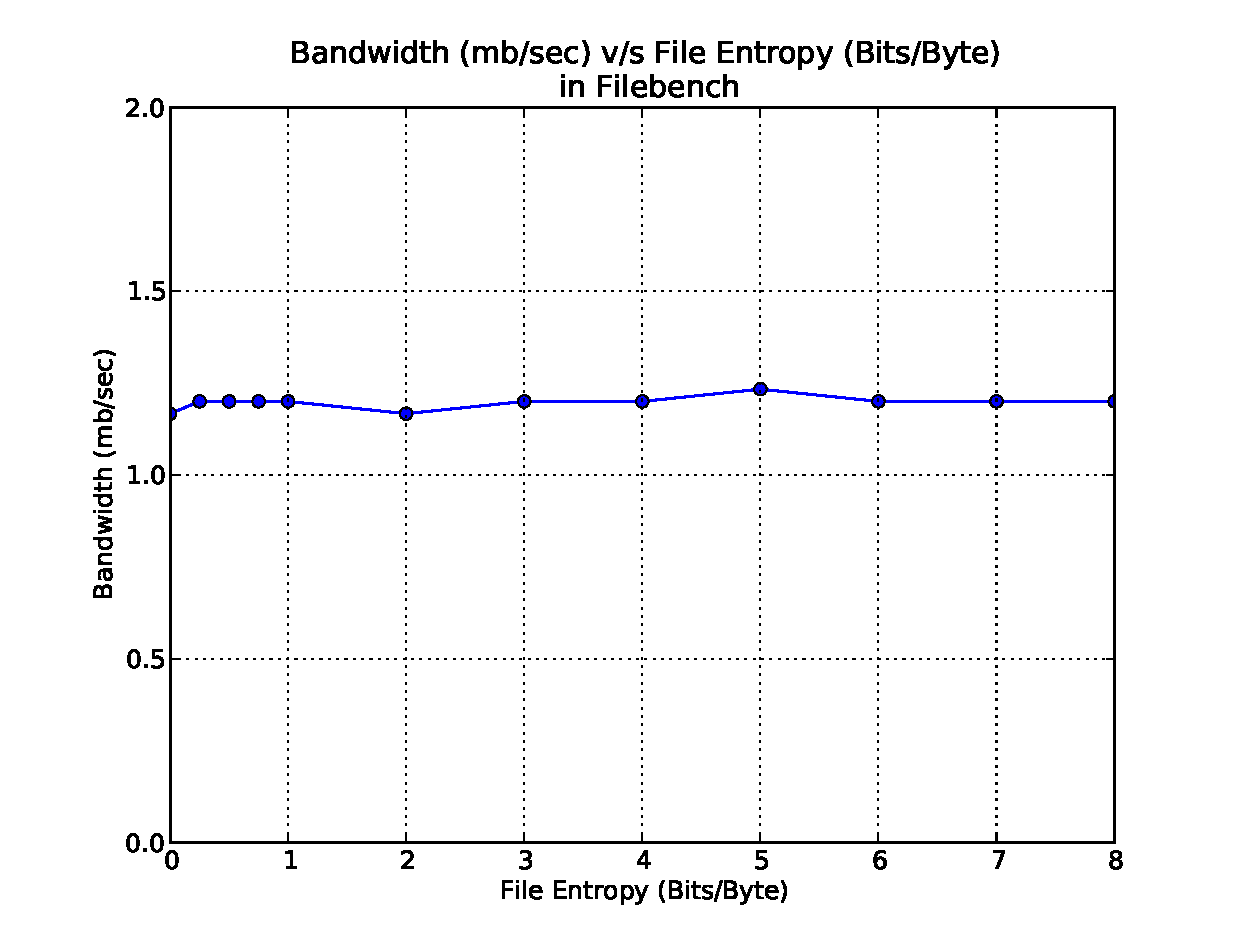
\includegraphics[scale=.55]{../results/set2/write_bw_avg_2.eps}
\caption{The average bandwidth over all the different write runs}
\label{fig:wbavg2}
\end{center}
\end{figure}

\noindent Figure \ref{fig:wb2} and \ref{fig:wbavg2} show that the bandwidth of the write operation dropped dramatically to low values compared to the values using \verb+entropy_cont_fill+. This behavior can be explained based on the idea that the new method takes 3 times the time required by the first method to generate the data which makes the disk idle most of the time, so the average bandwidth achieved is so low. Moreover, the lookup generates random data with homogeneous entropy over the file which makes it so hard for the SDFS to find deplicates chunks in the fileset.

\subsection{Writes: Latency v/s Entropy}
\begin{figure}[H]
\begin{center}
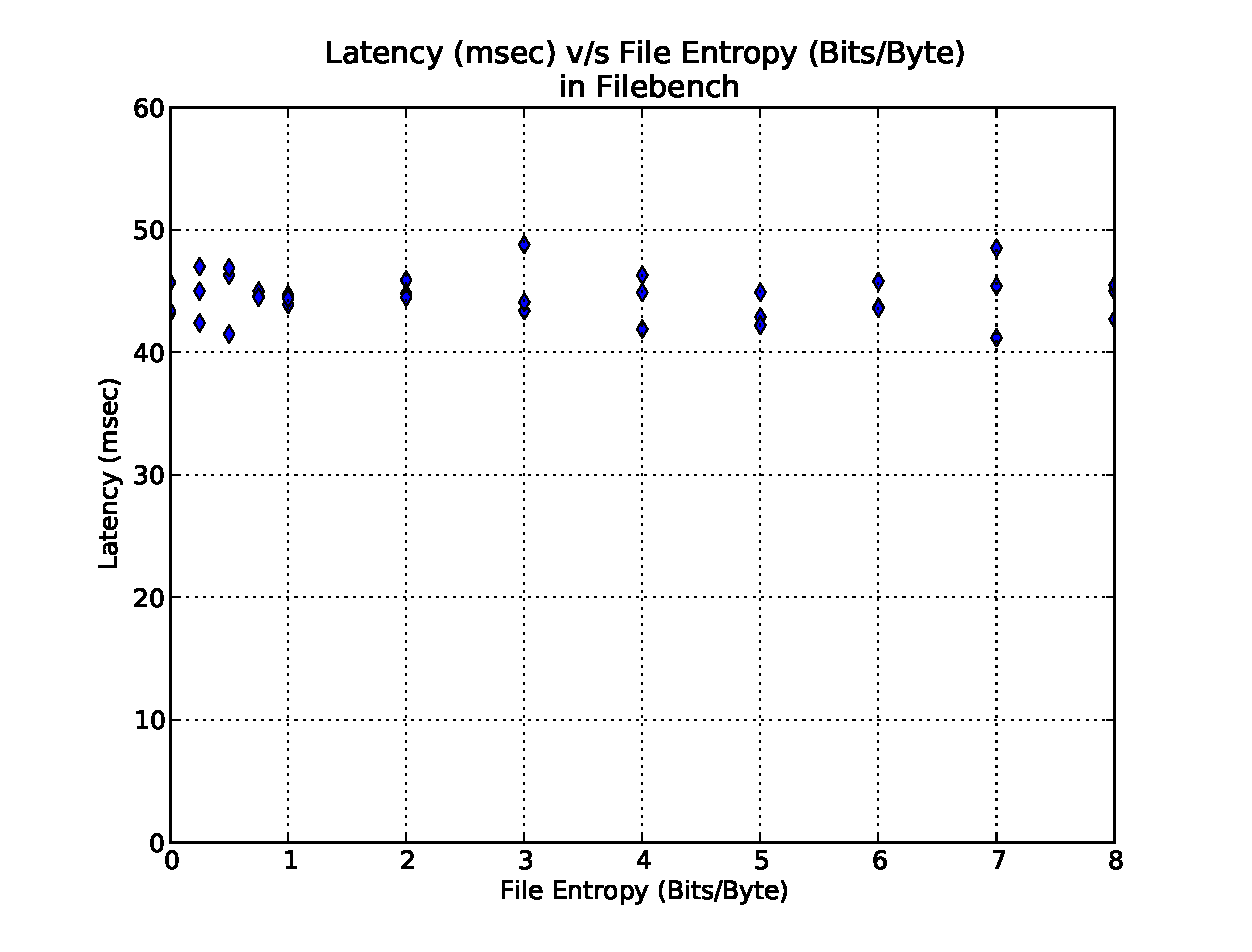
\includegraphics[scale=.55]{../results/set2/write_latency_2.eps}
\caption{The latency of all the different write runs}
\label{fig:wl2}
\end{center}
\end{figure}


\begin{figure}[H]
\begin{center}
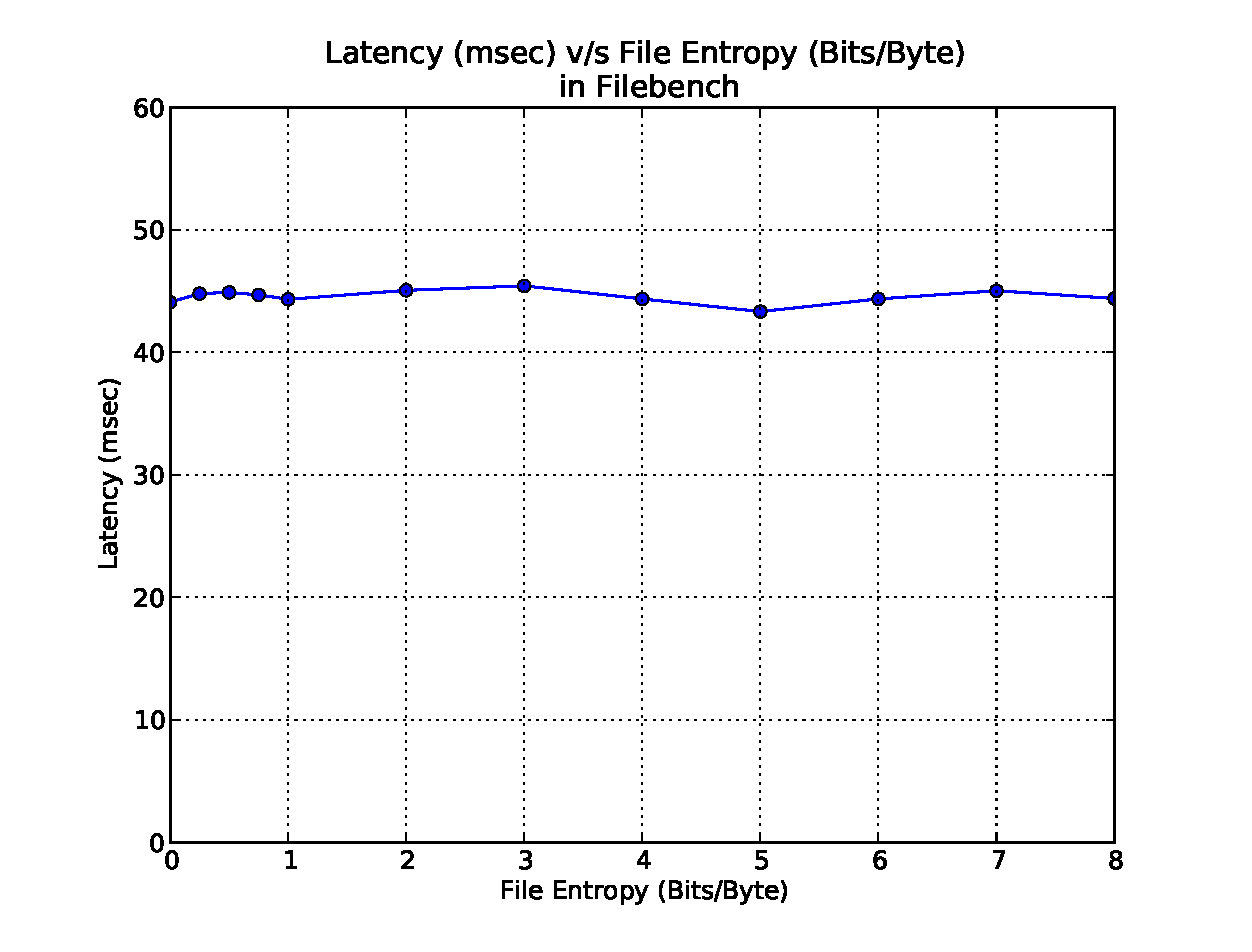
\includegraphics[scale=.55]{../results/set2/write_latency_avg_2.eps}
\caption{The average latency over all the write runs}
\label{fig:wlavg2}
\end{center}
\end{figure}
The results in these graphs are not as expected. Based on the premise that the newer method of entropy generation is slower, we expected the latency values to be higher than those achieved in the previous method. However, we do not have a convincing argument to explain these results and hence we cannot hypothesize about the reasons for these and for now, we leave them for future investigation.

\subsection{Writes: Operations/sec v/s Entropy}
\begin{figure}[H]
\begin{center}
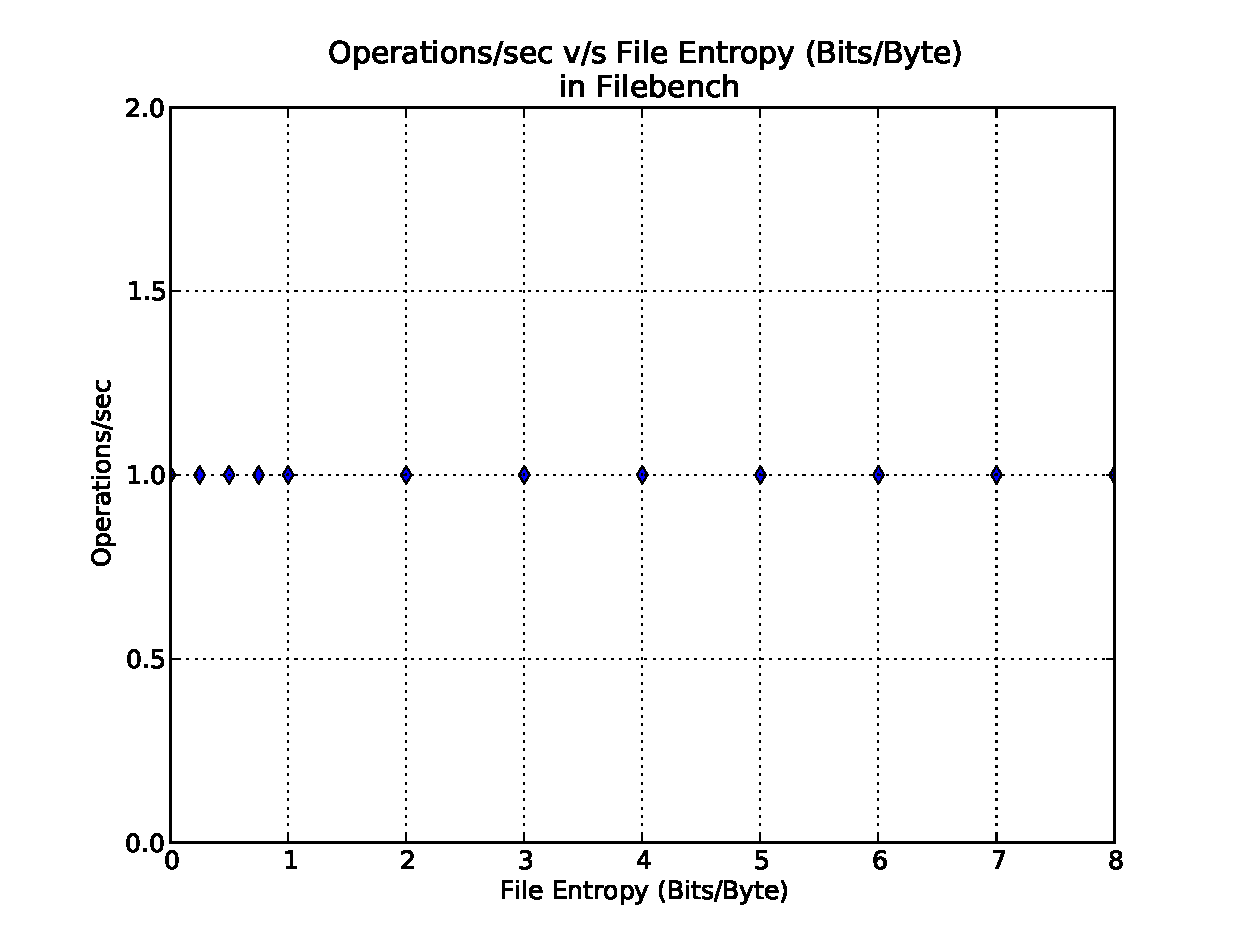
\includegraphics[scale=.55]{../results/set2/write_ops_2.eps}
\caption{The operations execution-speed of all the write runs}
\label{fig:wops2}
\end{center}
\end{figure}


\begin{figure}[H]
\begin{center}
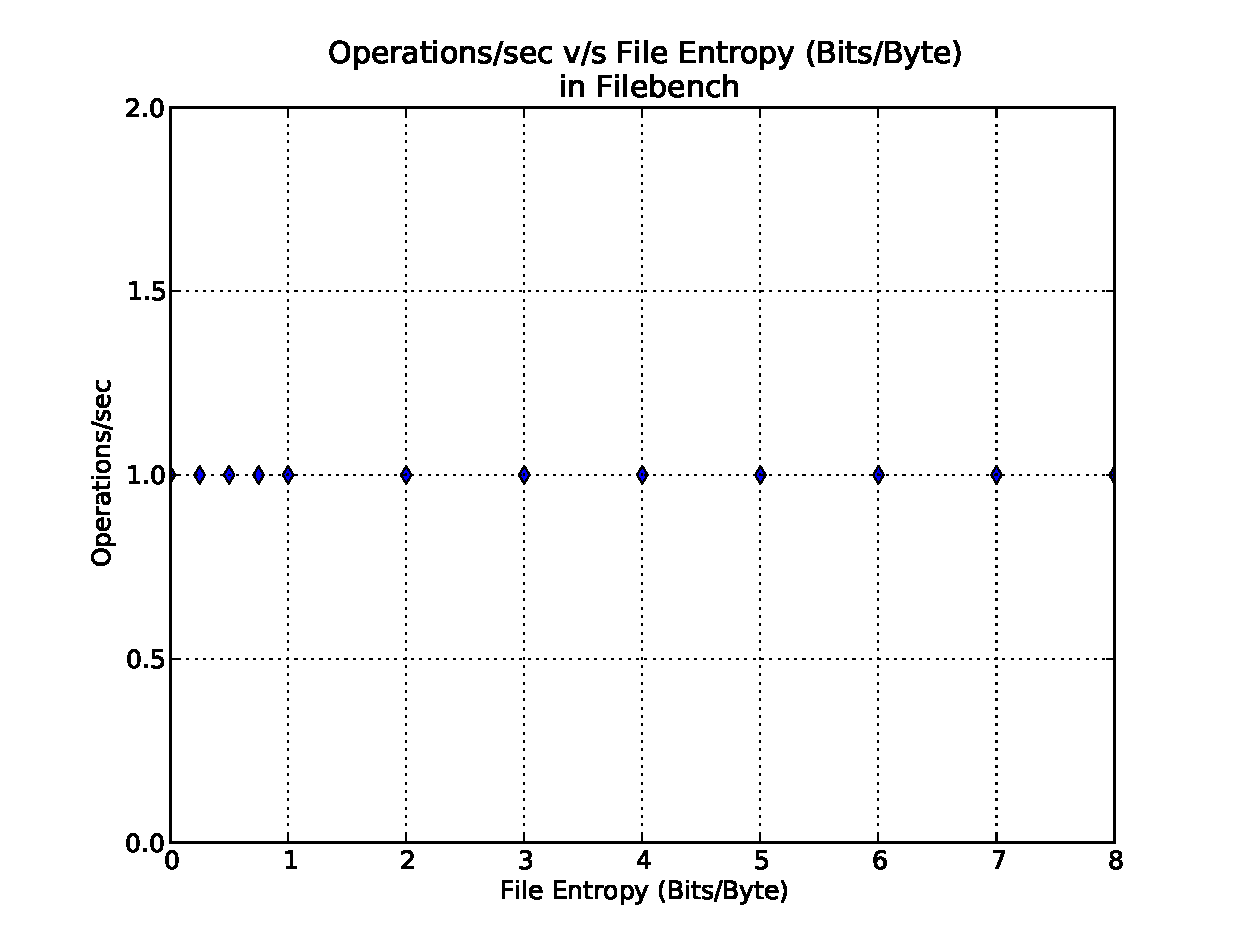
\includegraphics[scale=.55]{../results/set2/write_ops_2.eps}
\caption{The average operations execution-speed over all the write runs}
\label{fig:wopsavg2}
\end{center}
\end{figure}
The results achieved here are similar to Bandwidth and can explained based on the same ideas.

\subsection{Writes: Compression v/s Entropy}
\begin{figure}[H]
\begin{center}
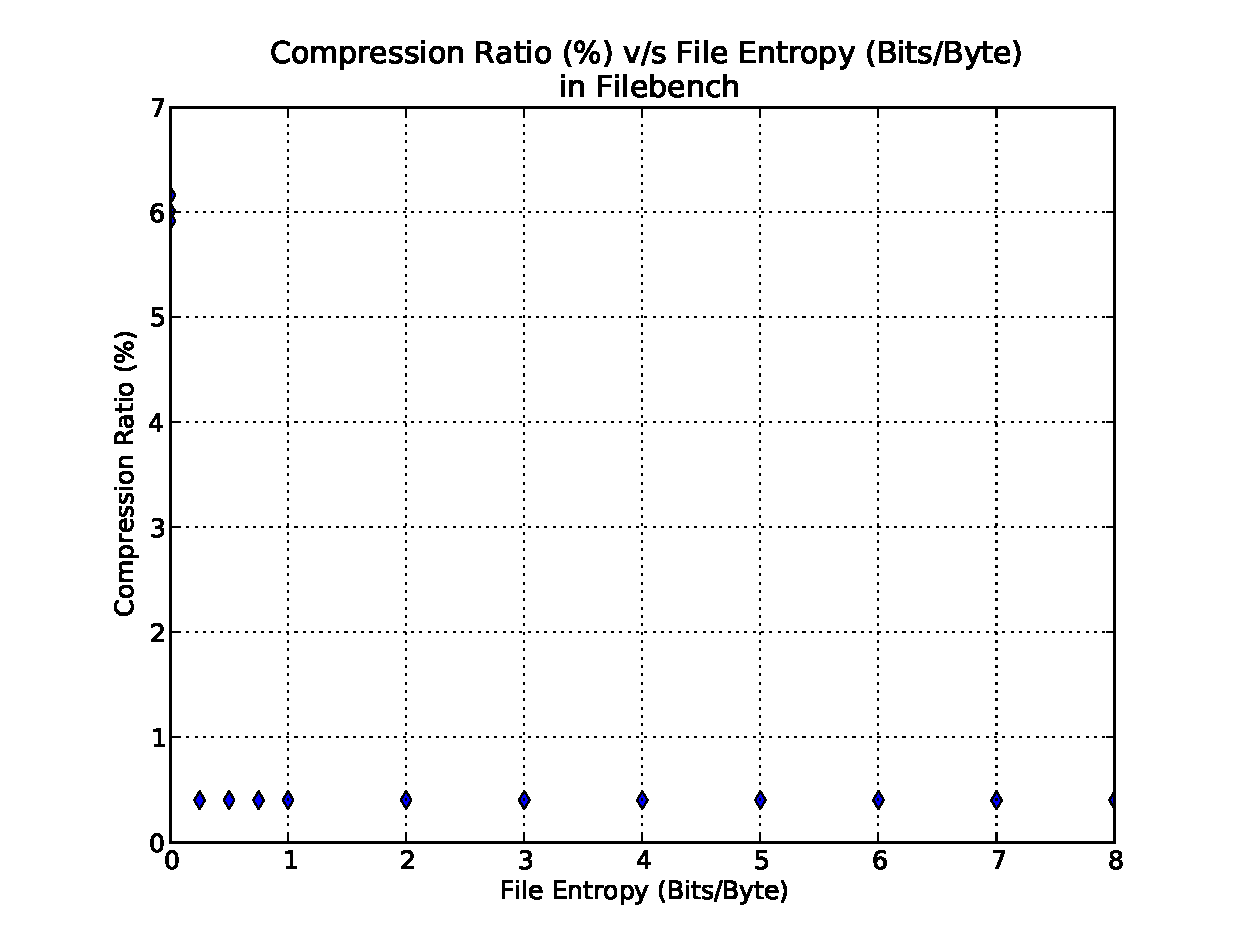
\includegraphics[scale=.55]{../results/set2/write_comp_2.eps}
\caption{The compression ratio of all the write runs}
\label{fig:comp2}
\end{center}
\end{figure}


\begin{figure}[H]
\begin{center}
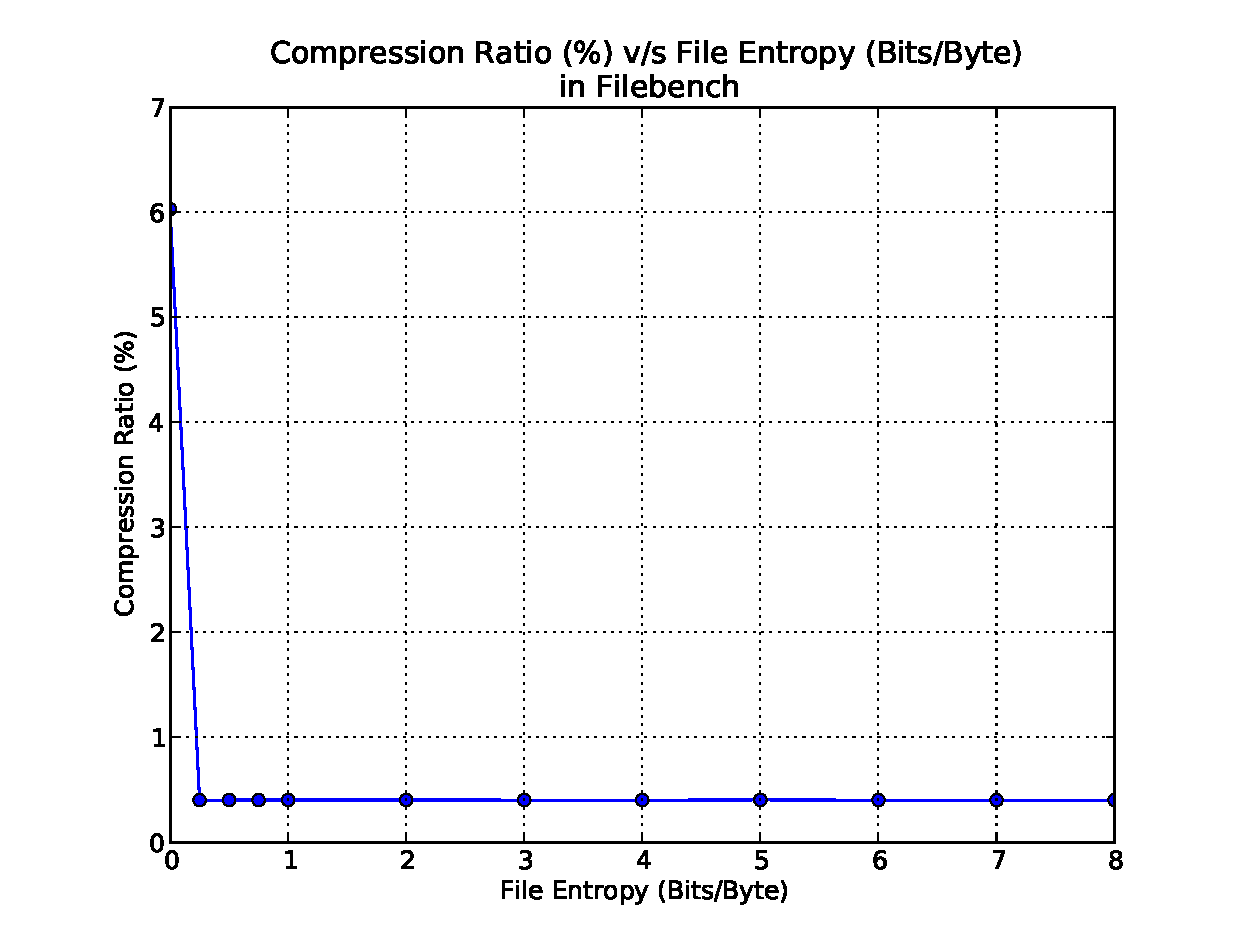
\includegraphics[scale=.55]{../results/set2/write_comp_avg_2.eps}
\caption{The compression ratio average over all the write runs}
\label{fig:compavg2}
\end{center}
\end{figure}

In Figures \ref{fig:comp2} and \ref{fig:compavg2} we see that as entropy is increased, compression levels decrease. As entropy is increased, the number of duplicate chunks on the disk become fewer and hence deduplication is not as effective anymore.

\chapter{Conclusions}\label{chap:conc}
\noindent We successfully implemented a mechansim in Filebench to incorporate entropy based data generation that can take arbitrary values that the user can specify in the range 0.0 to 8.0. We designed our implementation in such a way as to accomodate any future ways of specifying data and in doing so, made it easily extensible. We provide 5 ways of generating entropy, and each one differs in the amount of randomness that is generated. We provide a choice of using any of these methods to better benchmark deduplicating filesystems.
\newline
\noindent We showed that using entropy-based data generation, various metrics of a deduplicating filesystem can be studied better against different entropy values of the data that is actually written to or read from such a filesystem.

\chapter{Future Work}\label{chap:fut}
We realized a tradeoff between generating random data and performing read/write operations. While generating data takes a lot of time, except for the contiguous method explained in section \ref{sec:ent_imp}, this makes the processor lags behind the disk, which keeps the disk idle. However, this should not affect the results when we compare the readings obtained from different levels of an entropy used with a deduplication file system.
 However, testing other non-deduplication filesystems with entropy generation enabled will cause unexpected results because of the way the statistics are collected in Filebench.
\newline
\noindent Filebench calculates the averages bandwidth and operations per second.
 Therefore, if the entropy is enabled while running filebench on ext2 for example, most of the time the disk will be idle which will result in lower readings than the case if entropy is switched off, although ext2 is not aware of the data that is being written the previous scenario 
\newline
\noindent To fix this, Filebench has to be modified to calculate the time the disk is actually used and use only that time to calculate the average bandwidth and operations per second.
\newline
\noindent Another point to mention is the model we are using to model practical loads. We are using entropy as the only characteristics of the file that is actually varied.
 Moreover, it is the same value across all the files. In normal loads like the ones in cloud computing servers where there is a lot of backups and snapshots, the entropy can high per file but the redundancy is also high.
 Using true randomization makes it so hard to generate any chunk of the file twice.
 Maybe it is better to generate a more realistic model by profiling large amount of storage and construct the PDF from that data. We can use such PDF to to calculate the probability that a page will be redundant to one already have been written on the disk.
